\documentclass[11pt,a4paper,titlepage]{article}
\usepackage[brazil]{babel}
\usepackage[utf8]{inputenc}
\usepackage[T1]{fontenc}

\newcommand{\titulo}{\textit{Relatório V - Pipeline}}

\newcommand{\cabecalho}{\textit{Relatório V}}

\usepackage{fancyhdr}
\usepackage{indentfirst}
\usepackage{setspace}
\usepackage{graphicx,url}
\usepackage[section]{placeins}
%\usepackage{color,colortbl}
\usepackage{amsmath}
\usepackage{amssymb}
\usepackage{amsthm}
\usepackage{wrapfig}
\usepackage{times}
\usepackage{hyphenat}
\usepackage{ae}
\usepackage{algorithm}
\usepackage[sort,numbers]{natbib}
%package to insert codes
\usepackage{listings}
\usepackage{mips}
\usepackage{tabularx}
\usepackage{makecell}
%appendix
\usepackage[titletoc,toc,page]{appendix}
\renewcommand{\appendixtocname}{Apêndices}
\renewcommand{\appendixpagename}{Apêndices}

% the following is needed for syntax highlighting
\usepackage{color}

\definecolor{dkgreen}{rgb}{0,0.6,0}
\definecolor{gray}{rgb}{0.5,0.5,0.5}
\definecolor{mauve}{rgb}{0.58,0,0.82}

\lstset{ %código assembly
  language=[mips]Assembler,       % the language of the code
  basicstyle=\footnotesize,       % the size of the fonts that are used for the code
  numbers=left,                   % where to put the line-numbers
  numberstyle=\tiny\color{gray},  % the style that is used for the line-numbers
  stepnumber=1,                   % the step between two line-numbers. If it's 1, each line 
                                  % will be numbered
  numbersep=5pt,                  % how far the line-numbers are from the code
  backgroundcolor=\color{white},  % choose the background color. You must add \usepackage{color}
  showspaces=false,               % show spaces adding particular underscores
  showstringspaces=false,         % underline spaces within strings
  showtabs=false,                 % show tabs within strings adding particular underscores
  frame=single,                   % adds a frame around the code
  rulecolor=\color{black},        % if not set, the frame-color may be changed on line-breaks within not-black text (e.g. commens (green here))
  tabsize=4,                      % sets default tabsize to 2 spaces
  captionpos=b,                   % sets the caption-position to bottom
  breaklines=true,                % sets automatic line breaking
  breakatwhitespace=false,        % sets if automatic breaks should only happen at whitespace
  title=\lstname,                 % show the filename of files included with \lstinputlisting;
                                  % also try caption instead of title
  keywordstyle=\color{blue},          % keyword style
  commentstyle=\color{dkgreen},       % comment style
  stringstyle=\color{mauve},         % string literal style
  escapeinside={\%*}{*)},            % if you want to add a comment within your code
  morekeywords={*,...}               % if you want to add more keywords to the set
}
\usepackage{xcolor}
\definecolor{vgreen}{RGB}{104,180,104}
\definecolor{vblue}{RGB}{49,49,255}
\definecolor{vorange}{RGB}{255,143,102}
%mostrar código do verilog
\lstdefinestyle{verilog-style}
{
    language=Verilog,
    basicstyle=\small\ttfamily,
    keywordstyle=\color{vblue},
    identifierstyle=\color{black},
    commentstyle=\color{vgreen},
    numbers=left,
    numberstyle=\tiny\color{black},
    numbersep=10pt,
    tabsize=8,
    moredelim=*[s][\colorIndex]{[}{]},
    literate=*{:}{:}1
}

\makeatletter
\newcommand*\@lbracket{[}
\newcommand*\@rbracket{]}
\newcommand*\@colon{:}
\newcommand*\colorIndex{%
    \edef\@temp{\the\lst@token}%
    \ifx\@temp\@lbracket \color{black}%
    \else\ifx\@temp\@rbracket \color{black}%
    \else\ifx\@temp\@colon \color{black}%
    \else \color{vorange}%
    \fi\fi\fi
}
\makeatother

\usepackage{trace}

% Criar figura dividida em subfiguras
\usepackage{subfigure}

\usepackage{subfig}
\usepackage{ae}
\usepackage{aecompl}

\usepackage{multirow}
%\usepackage{epstopdf}

\pagestyle{fancy}

\setlength{\evensidemargin}{0.0in}
\setlength{\oddsidemargin}{0.0in}
\setlength{\textwidth}{6.6in}
\setlength{\textheight}{1.06\textheight}

\lhead{}
\chead{}
\rhead{\footnotesize{\textsc{\cabecalho}}}
\lfoot{\footnotesize{Iuri Silva Castro, João Mateus de Freitas Veneroso, Ricardo Pagoto Marinho}}
\cfoot{}
\rfoot{\footnotesize{\thepage}}
\setlength{\headwidth}{\textwidth}
\renewcommand{\headrulewidth}{0.4pt}
\renewcommand{\footrulewidth}{0.4pt}
\renewcommand{\baselinestretch}{0.90}

%\hyphenation{ ca-rac-te-ri-zan-do--se }

\begin{document}

\begin{titlepage}
\begin{center}

\begin{large}
Universidade Federal de Minas Gerais\\
Instituto de Ciências Exatas\\
Departamento de Ciência da Computação\\
\end{large}

\vspace{20mm}

\begin{Large}
DCC819 - Arquitetura de Computadores
\end{Large}

\vspace{20mm}

\begin{LARGE}
\titulo
\end{LARGE}


\vspace{30mm}

\begin{Large}
\begin{center}
Iuri Silva Castro\\ João Mateus de Freitas Veneroso\\ Ricardo Pagoto Marinho \\
\end{center}
\end{Large}


\vspace{60mm}

{\sc Belo Horizonte - MG}

{\sc \today}

%\vspace{10mm}
\end{center}
\end{titlepage}

\section{Introdução}\label{sec:desc}

O \textit{pipeline} é uma técnica de \textit{hardware} para promover paralelismo à nível de instrução dentro de um processador. O objetivo da técnica é dividir a execução da instrução em estágios, de forma que, quando a instrução termina o estágio, a próxima já pode ser processada por esse estágio, mantendo então todos os estágios do processador ocupados com alguma instrução pelo máximo de tempo possível. Essa técnica se assemelha a uma linha de montagem, permitindo aumentar consideravelmente o \textit{throughput} do processador em comparação à execução puramente sequencial, pois várias tarefas podem ser executadas em um mesmo ciclo de \textit{clock}.

No entanto, a técnica de \textit{Pipelining} complexifica o controle do processador, uma vez que a execução paralela introduz \textit{Hazards} no caminho de dados, que não existiriam no caso da execução sequencial, como:

\begin{itemize}

\item \textit{Hazards Estruturais}: restrições no número de instruções que podem utilizar um módulo do processador ao mesmo tempo, pois apenas uma intrução pode utilizar uma unidade funcional por vez. Pode ser amenizado com o aumento do número de unidades funcionais;

\item \textit{Hazards de Dados}: dependência de dados entre instruções. A instrução depende do resultado de uma instrução que ainda não terminou de executar. Pode ser amenizado com técnicas de encaminhamento de dados dentro dos estágios da pipeline;

\item \textit{Hazards de Controle}: instruções que fazem desvio do fluxo do programa, alterando o Contador de Programa (\textit{Program Counter}), tornam as próximas instruões indefinidas até que o novo valor do \textit{Program Counter} seja definido/calculado. Pode ser amenizado com técnicas de previsão de \textit{branches}.

\end{itemize}

Os \textit{Hazards}, quando ocorrem, necessitam que seja introduzido no fluxo do \textit{pipeline} bolhas, ou \textit{stalls}, para resolver esses conflitos.

Para este trabalho, propõe-se a implementação de um \textit{Pipeline} de três estágios sobre o caminho de dados implementado nos trabalhos anteriores. O processador de 16-bits finalizado faz encaminhamento de dados e gera dois ciclos de \textit{stall} ao executar instruções de \textit{branch} e \textit{jump}.

\section{Descrição}\label{sec:desc}

Nessa seção, descreve-se a organização e a arquitetura do processador proposto neste trabalho.

\subsection{Organização}

O processador desenvolvido nos trabalhos anteriores possuia 5 estágios de execução, sendo, busca de instrução, decodificação, busca de registradores, execução e armazenamento de resultados. Cada estágio requeria um passo de relógio, ou uma transição do sinal de \textit{clock}, e não possuia qualquer paralelismo a nível de instrução.

Para a implementação do \textit{pipeline}, propôs-se uma divisão do processador em 3 estágios: decodificação, execução e armazenamento de resultados. A Figura \ref{fig:pipeline3stage} abaixo mostra a divisão dos estágios.

\begin{figure}[!h]
\centering
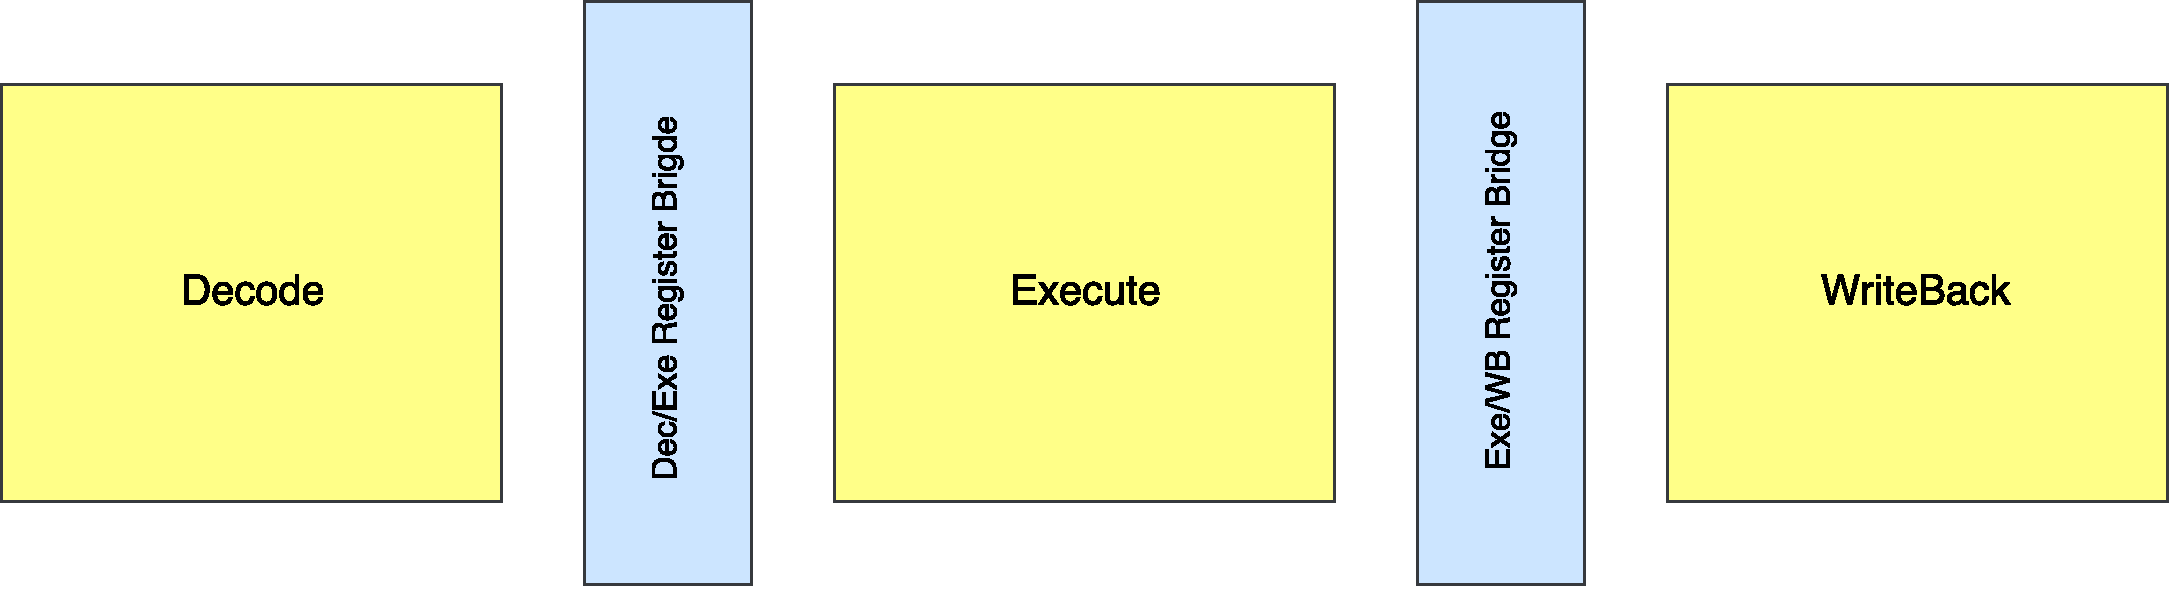
\includegraphics[scale=0.4]{images/pipeline.pdf}
\caption{Estrutura de \textit{pipeline} de 3 estágios proposta.}
\label{fig:pipeline3stage}
\end{figure}

Entre os estágios estão as \textit{register bridges}, ou registradores de ponte, que são utilizados para passar as informações e sinais de controle de um estágio para o outro. Os estágios, então, serão responsáveis pelas seguintes tarefas:

\begin{itemize}
\item \textit{Decode}: busca de instrução e decodificação de instrução;
\item \textit{Execute}: busca de registros e execução;
\item \textit{WriteBack}: escrita de resultados.
\end{itemize}

Para aplicação do \textit{pipeline} necessita-se que os estágios utilizem o mesmo tempo de execução, assim cada estágio executa em duas transições do sinal de \textit{clock}, mesmo o estágio de \textit{WriteBack} que ficará então uma transição \textit{idle} para adequar ao tempo dos outros estágios.

O \textit{pipeline} insere no sistema \textit{Hazards}, como descrito anteriormente, e para isso precisa-se utilizar de algumas técnicas para eliminar ou amenizar o problema. Eliminou-se o \textit{hazard} de dados utilizando a técnica de encaminhamento, assim dados que são encaminhados da saída do estágio de execução para a entrada do mesmo estágio, não havendo \textit{stalls}. O sistema não possui \textit{hazards} estruturais, pois todos os estágios requerem o mesmo tempo de execução e o \textit{Banco de Registradores} possui duas portas de leitura e uma de escrita. Além disso o estágio de execução possui uma unidade dedicada para executar multiplicações, conseguindo, assim, executar instruções de multiplicação em um ciclo. Para instruções de desvio de fluxo \textit{hazards} de controle acontecem, e são gerados dois \textit{stalls} quando tais instruções são detectadas.

\subsection{Arquitetura}

O conjunto final de instruções do processador está descrito na tabela \ref{tab:instructions}. Todas as instruções aritméticas e lógicas recebem o operando A do banco de registradores e o operando B pode ser um imediato de 4-bit ou um registrador, dependendo da instrução. A instrução \textit{BEZ} não utiliza os bits 11-8 e as instruções \textit{GHI} e \textit{GLO} não utilizam os bits de 7-0. A instrução \textit{J} altera o \textit{PC} para um valor imediato de 12-bit que comporta qualquer endereço da memória de 4096 posições.

\begin{table}[!h]
\centering
\begin{tabular}{| c | c | c | c | c | l |}
\hline
Instrução & Opcode & Bits 11-8 & Bits 7-4 & Bits 3-0 & Descrição \\
\hline
 ADD  & 0000 & C & B & A   & Reg(C) = Reg(A) + Reg(B) \\
\hline
 SUB  & 0001 & C & B & A   & Reg(C) = Reg(A) - Reg(B) \\
\hline
 SLTI & 0010 & C & Imm & A & Reg(C) = Reg(A) > Imm \\
\hline
 AND  & 0011 & C & B & A   & Reg(C) = Reg(A) AND Reg(B) \\
\hline
 OR   & 0100 & C & B & A   & Reg(C) = Reg(A) OR Reg(B) \\
\hline
 XOR  & 0101 & C & B & A   & Reg(C) = Reg(A) XOR Reg(B) \\
\hline
 ANDI & 0110 & C & Imm & A & Reg(C) = Reg(A) + Imm \\
\hline
 ORI  & 0111 & C & Imm & A & Reg(C) = Reg(A) OR Imm \\
\hline
 XORI & 1000 & C & Imm & A & Reg(C) = Reg(A) XOR Imm \\
\hline
 ADDI & 1001 & C & Imm & A & Reg(C) = Reg(A) + Imm \\
\hline
 SUBI & 1010 & C & Imm & A & Reg(C) = Reg(A) - Imm \\
\hline
 J    & 1011 & \multicolumn{3}{c|}{Imm} & PC = Imm \\
\hline
 BEZ  & 1100 & - & B & A   & If (Reg(A) = 0) PC = Reg(B) \\
\hline
 MUL  & 1101 & C & B & A   & Reg(C) = Reg(A) * Reg(B) \\
\hline
 GHI  & 1110 & C & - & -   & Reg(C) = HI \\
\hline
 GLO  & 1111 & C & - & -   & Reg(C) = LO \\
\hline
\end{tabular}
\caption{Instruções}
\label{tab:instructions}
\end{table}
\captionsetup{font={footnotesize,rm},justification=centering,labelsep=period}%

\section{Implementação}

\begin{figure}[!h]
\centering
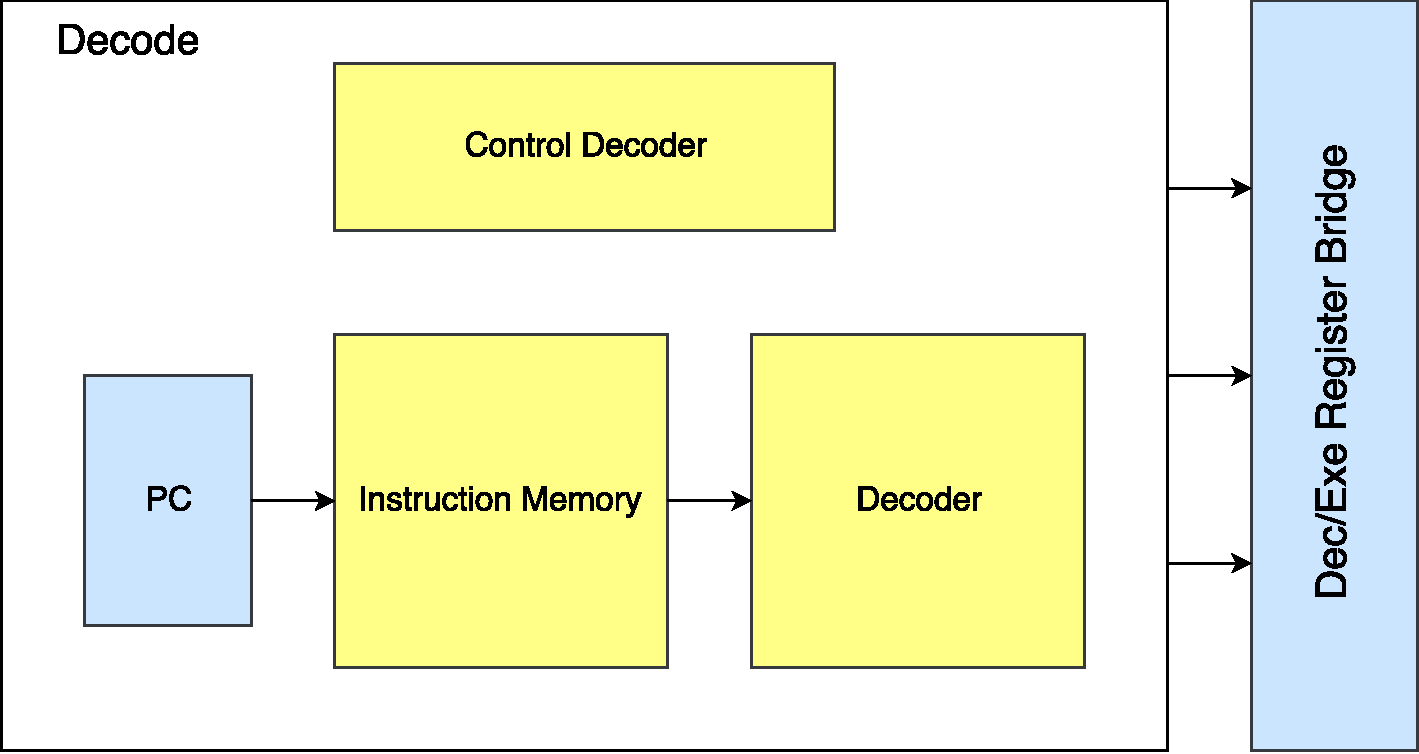
\includegraphics[scale=0.4]{images/decodepipe.pdf}
\caption{Diagrama simplificado do estágio \textit{Decode} do \textit{pipeline}.}
\label{fig:decodepipe}
\end{figure}

\begin{figure}[!h]
\centering
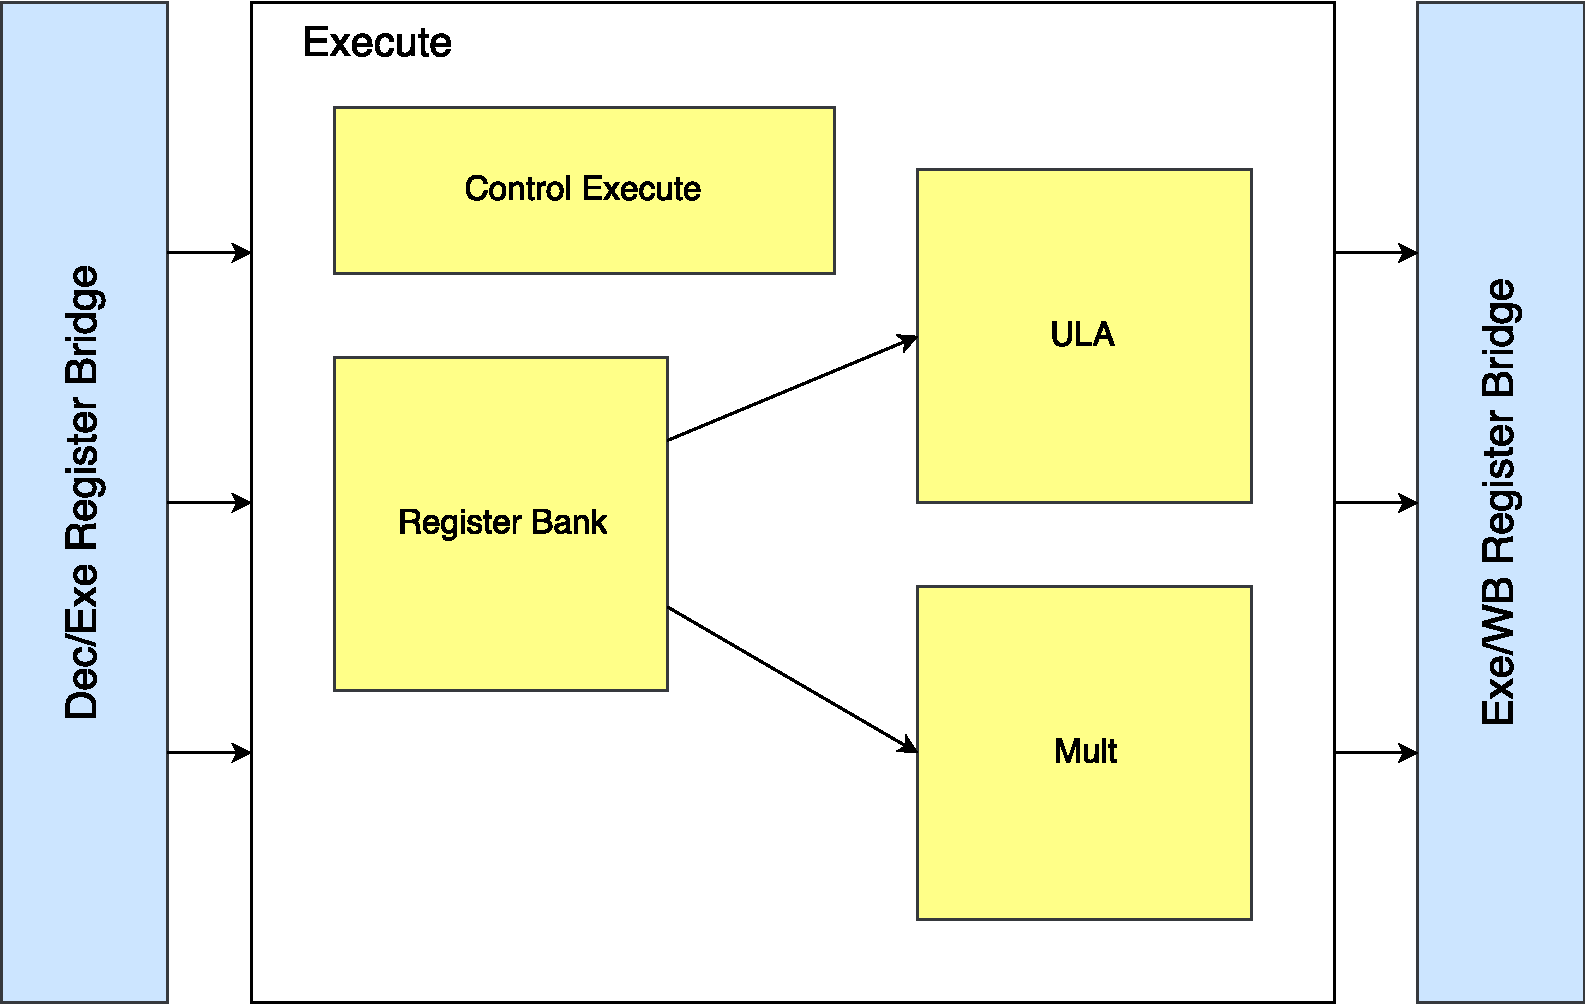
\includegraphics[scale=0.4]{images/executepipe.pdf}
\caption{Diagrama simplificado do estágio \textit{Execute} do \textit{pipeline}.}
\label{fig:executepipe}
\end{figure}

\begin{figure}[!h]
\centering
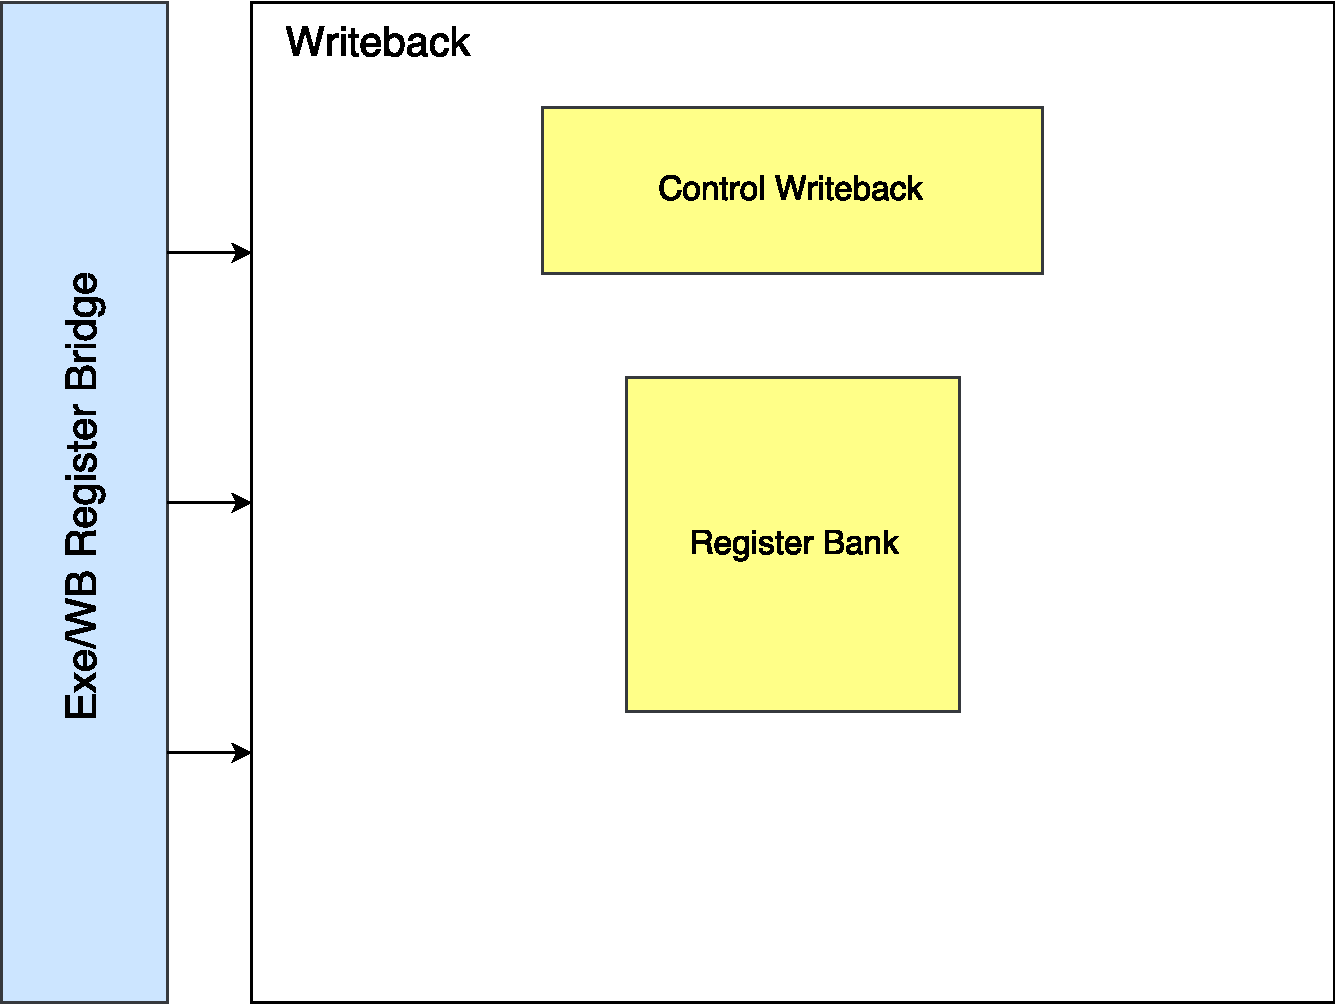
\includegraphics[scale=0.4]{images/writebackpipe.pdf}
\caption{Diagrama simplificado do estágio \textit{Writeback} do \textit{pipeline}.}
\label{fig:writebackpipe}
\end{figure}

O processador finalizado conta com quatro módulos principais, além de uma série de módulos
de controle secundários e multiplexadores. Os módulos principais são:

\begin{itemize}

\item \textit{Decoder}: recebe a instrução de 16 bits e decodifica o \textit{Opcode},
identificando os operandos e preparando os registradores que sinalizam se a instrução é uma 
multiplicação, se é um \textit{Jump}, se haverá \textit{Stall}, se haverá \textit{Write Back},
qual registrador da multiplicação será armazenado se for o caso e se o segundo operando é
um imediato.

\item \textit{Register Bank}: o banco de registradores conta com 16 registradores de 16 bits,
duas portas de leituras para os operandos A e B e uma porta de escrita.

\item \textit{Unidade Lógica Aritmética}: a unidade lógica aritmética executa as instruções: 
ADD, SUB, SLT, AND, OR, XOR e BEZ.

\item \textit{Unidade multiplicadora}: a unidade multiplicadora recebe dois operandos de 16-bits
e executa uma multiplicação produzindo um resultado de 32-bits que é armazenado em dois registradores:
HI, que armazena os 16-bits mais significativos e LO, que armazena os 16-bits menos significativos.
O resultado da operação armazenado nos registradores pode ser acessado por meio das instruções 
GHI e GLO, que escrevem o conteúdo dos registradores HI e LO, respectivamente, em um registrador
do banco de registradores.

\end{itemize}



\section{Integração}

\begin{figure}[!h]
\centering
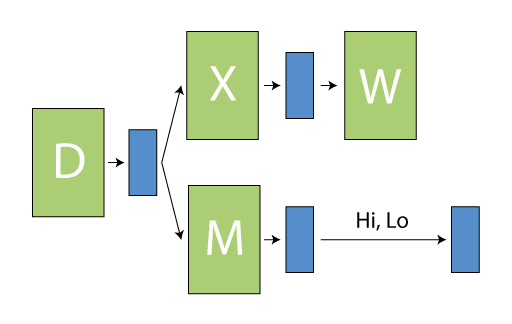
\includegraphics[scale=0.5]{images/pipeline_diagram.png}
\caption{Diagrama da \textit{pipeline}}
\label{fig:pipeline_diagram}
\end{figure}

A pipeline implementada possui três estágios: Decodificação, Execução e \textit{Write Back}.
O estágio de execução é dividido entre dois módulos independentes: o módulo de multiplicação e a 
Unidade Lógica Aritmética. O diagrama na figura \ref{fig:pipeline_diagram} descreve a \textit{pipeline}.

Cada um dos estágios da \textit{pipeline} tem uma máquina de estados associada que executa as operações
necessárias em múltiplos ciclos de \textit{clock}. Ao fim de cada estágio, cada módulo
define os valores de um conjunto de registradores que passa os dados para o próximo estágio por
meio de um \textit{buffer}. Na nossa implementação existem dois \textit{buffers}: Decode/Execute
e Execute/Write Back.

O estágio \textit{Decoder} (D) recebe a próxima instrução da memória de instruções e define 
os valores dos registradores a seguir com base no \textit{Opcode} da instrução, atualizando
o \textit{buffer} Decode/Execute:

\begin{itemize}
\item OpULA: o opcode da instrução para a ULA com 4-bits que indica a operação aritmética 
a ser realizada. Por exemplo: ADDI e ADD tem o mesmo OpULA.
\item OpA, OpB, OpC: os operandos A, B e C.
\item IsImm: indica se o segundo operando da instrução é um imediato.
\item IsJump: indica se a instrução é um \textit{Jump} (J).
\item HasWB: indica se a instrução faz \textit{Write Back}.
\item HasStall: indica se a instrução gera \textit{Stall}.
\item IsMult: indica se a instrução vai utilizar a unidade multiplicadora.
\item HiLo: indica qual registrador da multiplicação vai ser armazenado.
\item StoreHiLo: indica que vai armazenar um registrador da unidade multiplicadora.
\item AddrImm: endereço de memória de 12-bits para o \textit{Jump}.
\end{itemize}

O estágio \textit{Execução} (X e M) pode ocorrer em dois módulos separados: a ULA e a unidade
multiplicadora. As entradas dos módulos são os registradores de saída da etapa anterior
descritos acima. O resultado da ULA é armazenado no registrador Res e as flags da operação
são armazenadas no registrador FlagReg. Já a unidade de multiplicação produz um resultado
que é armazenado nos registradores Hi e Lo de 16-bits. O \textit{buffer} Execute/Write Back
conta com os seguintes registradores:

\begin{itemize}
\item Res: indica o resultado da operação na ULA ou os registradores Hi ou Lo da unidade multiplicadora.
\item FlagReg: indica as flags da ULA.
\item RegDest: indica o registrador de destino da operação de \textit{Write Back}.
\item HasWB: indica se o \textit{Write Back} vai ser executado.
\item AddrImm: indica o endereço do imediato da operação \textit{Jump} (J).
\item HasJumped: indica se um \textit{Jump} foi executado.
\item HasStall: indica se houve \textit{Stall}.
\end{itemize}

Um multiplexador redireciona a saída da ULA e da unidade multiplexadora para o estágio de 
\textit{WriteBack}. Perceba que a operação de multiplicação não passa efetivamente pelo estágio de 
\textit{WriteBack} uma vez que o resultado da operação fica armazenado apenas nos registradores Hi
e Lo, que podem ser escritos no banco de registradores por meio da execução de mais duas 
instruções: GHI e GLO.

\section{Simulação e Testes}

Os testes realizados procuraram medir a melhora de desempenho após a implementação da \textit{pipeline}.
Para isso, um programa de teste foi executado no processador antigo sem \textit{pipeline} e no processador
novo com a \textit{pipeline} de três estágios. Perceba que a ordem dos operandos está invertida no
\textit{Assembly}. Isso ocorre porque no nosso processador o operando 2, que pode ser um imediato, é o
operando referente aos bits 7-4 da instrução e não 3-0. Portanto, o código foi alterado para refletir
a característica das instruções armazenadas na memória.

\begin{table}[!h]
\centering
\begin{tabular}{| l | l |}
\hline
ADDI R1, 8, R0   &  R1 = 8                             \\
ADDI R2, 8, R0   &  R2 = 8                             \\
MUL  -, R2, R1   &  R1 * R2 = 64                       \\
GLO  R1, -, -    &  R1 = 64.                           \\
ADDI R2, 15, R0  &  R2 = 15.                           \\
ADDI R2, 1, R2   &  R2 = 15 + 1.                       \\
MUL  -, R1, R2   &  R1 * R2 = 1024.                    \\
GLO  R1, -, -    &  R1 = 1024.                         \\
ADDI R2, 10, R0  &  R2 = 10.                           \\
MUL  -, R2, R2   &  R2 * R2 = 100.                     \\
GLO  R2, -, -    &  R2 = 100.                          \\
ADDI R3, 0, R1   &  R3 = R1 = 1024.                    \\
ADDI R4, 0, R0   &  R4 = 0.                            \\
ADDI R6, 15, R0  &  R6 = 15.                           \\
ADDI R6, 8, R6   &  R6 = 23.                           \\
ADDI R4, 1, R4   &  R4 = R4 + 1                        \\
SUB  R3, R2, R3  &  R3 = R3 - R2.                      \\
SLTI R5, 9, R4   &  R5 = R4 > 9                        \\
BEZ   -, R6, R5  &  If (R5 == 0) { jump to \#R6 }        \\
\hline
\end{tabular}
\caption{Programa de teste}
\label{tab:program}
\end{table}

O programa de teste realiza a divisão de 1024 por 100, calculando o resto por meio de um loop e armazenando 
o resultado no resgistrador R3. O programa está decrito na tabela \ref{tab:program}.

A figura XXX mostra o resultado da simulação no processador antigo e a figura YYY mostra o resultado da 
simulação no processador novo. Como percebemos pelos resultados, o processador novo executou o programa
em Y \textit{clocks} e o processador antigo executou o programa em X \textit{clocks}. Portanto, a
\textit{pipeline} obteve uma melhora de 99\% nesse caso específico.

Além deste, fizemos um programa para ordenar um vetor de 5 valores.
O código do programa está descrito a seguir.
Para melhor visualização e entendimento do código, ele foi dividido em blocos de 12 instruções.
Os blocos são equivalentes, o que muda são os valores dos registradores.

O vetor está armazenado nos registradores 11 a 15.
A cada bloco, o valor de um registrador é trocado com outro caso o seguinte seja menor do que ele.
As trocas começam no registrador 11 (R11) e vão até o 14 (R14).
No R11, primeiro verificamos se o valor de R12 é menor do que o dele, caso seja, troca os valores.
Então o mesmo processo é feito com o R13, R14 e R15.
Depois de finalizada as comparações do R11, olhamos para o R12 e fazemos o mesmo processo, \textit{i.e.}, comparamos primeiro com o R13, depois com o R14 e por último com o R15.
Este processo se repete até fazermos a última comparação de R14 e R15.
Após isso, o vetor está ordenado.

Devido ao limitado número de instruções disponíveis, algumas adaptações precisaram ser feitas.
A primeira é que não existe comparação de valores de registradores, logo para fazer isso, os valores a serem comparados são armazenados nos registradores R1 e R2.
Para saber se devemos trocar, fazemos a subtração desses valores e armazenamos em R3.
A partir daí, devemos saber se o número é positivo ou negativo.
Caso seja positivo, R2>R1 e a troca não deve acontecer.
Caso negativo, R2<R1 e a troca deve ocorrer.
Porém, a instrução de comparação SLTI não funciona com valores negativos, logo não podemos simplesmente comparar o valor de R3 com 0.
Para isso, utilizamos o registrador R9 que em seu bit mais significativo possui o valor 1 e nos demais o valor 0.
Com este registrador, fazemos um AND entre R9 e R3, dessa forma, sabemos o sinal de R3.
Agora podemos comparar R3 com 0 e descobrir se o resultado é positivo ou negativo.
Repare que caso R3=1, a subtração foi negativa, logo a troca deve ocorrer.
A decisão de se devemos ou não trocar os valores é armazenada em R4 que é utilizado em um \textit{branch}.
Se R4=0, então R3=0 e a troca não deve ocorrer, logo o \textit{branch} deve ser tomado.

Para realizar a troca, utilizamos o próprio R3 como registrador auxiliar.
Se o \textit{branch} precisar ser tomado, o programa pula para o valor armazenado em R8.
Para encontrar o valor de R8, utilizamos 3 registradores: R5, R6 e R7.
R5 armazena em qual bloco de 13 instruções estamos: no primeiro ele recebe o valor 1 e é incrementado em 1 a cada início de bloco.
R6 armazena a multiplicação de R5 e R7, cujo valor é 13 (tamanho do bloco de instruções).
Por fim, R8 pega os bits menos significativos da multiplicação e descobre para qual endereço deve pular caso necessário.

\begin{lstlisting}
ADDI R5,1,R0
ADDI R7,13,R0
MULL R6,R5,R7
GLO R8,-,-
ADD R1,R11,R0
ADD R2,R12,R0
SUB R3,R1,R2
AND R3,R9,R3 
SLTI R4,0,R3
BEZ -,R8,R4
ADD R3,R11,R0
ADD R11,R12,R0
ADD R12,R3,R0
# 2
ADDI R5,1,R5
ADDI R7,13,R0
MULL R6,R5,R7
GLO R8,-,-
ADD R1,R11,R0
ADD R2,R13,R0
SUB R3,R1,R2
AND R3,R9,R3
SLTI R4,0,R3
BEZ -,R8,R4
ADD R3,R11,R0
ADD R11,R13,R0
ADD R13,R3,R0
# 3
ADDI R5,1,R5
ADDI R7,13,R0
MULL R6,R5,R7
GLO R8,-,-
ADD R1,R11,R0
ADD R2,R14,R0
SUB R3,R1,R2
AND R3,R9,R3
SLTI R4,0,R3
BEZ -,R8,R4
ADD R3,R11,R0
ADD R11,R14,R0
ADD R14,R3,R0
# 4
ADDI R5,1,R5
ADDI R7,13,R0
MULL R6,R5,R7
GLO R8,-,-
ADD R1,R11,R0
ADD R2,R15,R0
SUB R3,R1,R2
AND R3,R9,R3
SLTI R4,0,R3
BEZ -,R8,R4
ADD R3,R11,R0
ADD R11,R15,R0
ADD R15,R3,R0
##### 5
ADDI R5,1,R5
ADDI R7,13,R0
MULL R6,R5,R7
GLO R8,-,-
ADD R1,R12,R0
ADD R2,R13,R0
SUB R3,R1,R2
AND R3,R9,R3 
SLTI R4,0,R3
BEZ -,R8,R4
ADD R3,R12,R0
ADD R12,R13,R0
ADD R13,R3,R0
# 6
ADDI R5,1,R5
ADDI R7,13,R0
MULL R6,R5,R7
GLO R8,-,-
ADD R1,R12,R0
ADD R2,R14,R0
SUB R3,R1,R2
AND R3,R9,R3 
SLTI R4,0,R3
BEZ -,R8,R4
ADD R3,R12,R0
ADD R12,R14,R0
ADD R14,R3,R0
# 7
ADDI R5,1,R5
ADDI R7,13,R0
MULL R6,R5,R7
GLO R8,-,-
ADD R1,R12,R0
ADD R2,R15,R0
SUB R3,R1,R2
AND R3,R9,R3 
SLTI R4,0,R3
BEZ -,R8,R4
ADD R3,R12,R0
ADD R12,R15,R0
ADD R15,R3,R0
##### 8
ADDI R5,1,R5
ADDI R7,13,R0
MULL R6,R5,R7
GLO R8,-,-
ADD R1,R13,R0
ADD R2,R14,R0
SUB R3,R1,R2
AND R3,R9,R3 
SLTI R4,0,R3
BEZ -,R8,R4
ADD R3,R13,R0
ADD R13,R14,R0
ADD R14,R3,R0
# 9
ADDI R5,1,R5
ADDI R7,13,R0
MULL R6,R5,R7
GLO R8,-,-
ADD R1,R13,R0
ADD R2,R15,R0
SUB R3,R1,R2
AND R3,R9,R3 
SLTI R4,0,R3
BEZ -,R8,R4
ADD R3,R13,R0
ADD R13,R15,R0
ADD R15,R3,R0
###### 10
ADDI R5,1,R5
ADDI R7,13,R0
MULL R6,R5,R7
GLO R8,-,-
ADD R1,R14,R0
ADD R2,R15,R0
SUB R3,R1,R2
AND R3,R9,R3 
SLTI R4,0,R3
BEZ -,R8,R4
ADD R3,R14,R0
ADD R14,R15,R04
ADD R15,R3,R0
\end{lstlisting}

A Figura~\ref{fig:ordena1} mostra como o vetor está distribuído nos registradores:
\begin{itemize}
\item R11 = 4
\item R12 = 3
\item R13 = 2
\item R14 = 5
\item R15 = 1
\end{itemize}

\begin{figure}[!h]
\centering
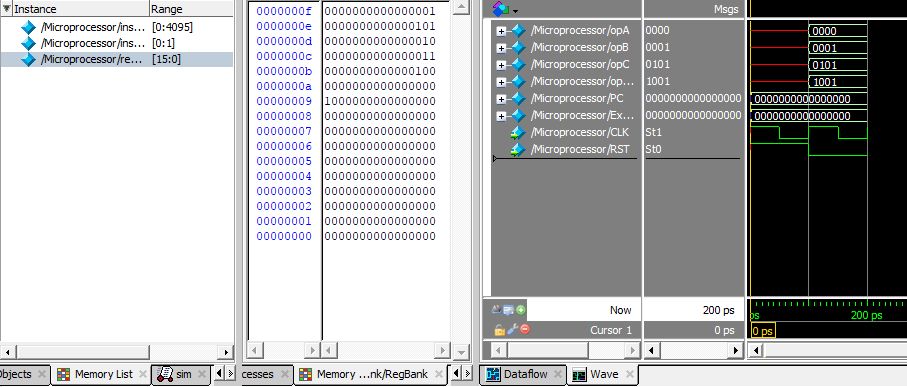
\includegraphics[scale=0.5]{images/ordena1.png}
\caption{Início da ordenação}
\label{fig:ordena1}
\end{figure}

Repare que R9 possui o bit mais significativo com valor 1 e os outros bits 0, como dito anteriormente.
A Figura~\ref{fig:ordena2} mostra o fim da simulação.
Note que o vetor está ordenado e que a simulação terminou com 28300 ps.


\begin{figure}[!h]
\centering
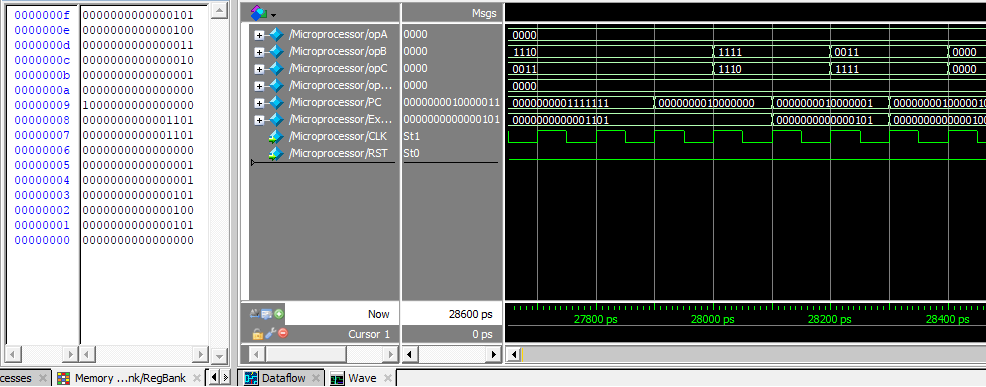
\includegraphics[scale=0.5]{images/ordena2.png}
\caption{Fim da ordenação}
\label{fig:ordena2}
\end{figure}
\section{Conclusão}

A incorporação da \textit{pipeline} de três estágios exigiu a introdução de \textit{buffers} e unidades de
controle adicionais no processador, complexificando consideravelmente o projeto. Os \textit{branches} exigiram
a introdução de um ciclo de \textit{stall} para esperar pelo novo \textit{Program Counter}, o que limitou
os ganhos de velocidade de execução. A lógica de encaminhamento foi implementada para evitar \textit{stalls}
devido à \textit{Hazards de dados}. Ao final, o ganho de desempenho obtido foi de cerca de 99\% no cenário de 
teste, o que mostra claramente a importância dos \textit{pipelines} em processadores de alto desempenho.

\bibliographystyle{unsrt}
\addcontentsline{toc}{section}{Referências}
%\bibliography{references}

\nocite{*}


\end{document}

